\documentclass[main.tex]{subfiles}
\begin{document}
\onlyinsubfile{\mainmatter{}}

\chapter{Glyco Heap-based Secure Calling Convention}
The previous chapter discussed the first milestone of the Glyco compiler, namely a nanopass compiler producing fairly traditional executables for CHERI-RISC-V targets, with almost no special considerations for capability machines, except for minor enhancements such as bounded heap-allocated buffers. This chapter discusses the first significant upgrade of the Glyco compiler, namely one where procedure calls are implemented using a secure \cc{} named \textbf{\ghscc{}} and adapted from the heap-based \cc{} proposed by \cite{cerise}.

We begin this chapter by describing the desired security properties of a \enquote{secure} \cc{} and listing some theoretical \ccs{} proposed in the literature that have those properties. We then describe the implementation of two runtime routines that form the basis of \ghscc{}, and how they interact with the new \cc{}. We finish with an evaluation of \ghscc{} against \gccc{} in terms of \lse{}, changes to the compiler and its \ils{}, generated codesize, and runtime performance.

% TODO: Move paragraph to implementation discussion
The \cc{} relies on a couple of runtime routines with access to capabilities not available to the user's source code. As Glyco is developed almost entirely in isolation, it cannot rely on an operating system or dynamic linker to provide these routines and therefore provides them itself. It is expected that a production compiler would be able to rely on an OS-provided standard library instead, thereby removing the need to trust the compiler.

\section{Background: Secure Calling Conventions}
A traditional \cc{} such as \gccc{} works with a single stack of call frames per thread, with each call frame holding a procedure call's ephemeral state, such as values assigned to local variables. When a procedure is called, a new call frame is pushed on the stack, the caller puts a return address in a designated register or location on the call frame, and passes control to the callee. When returning, the most recent call frame on the stack is popped and the callee jumps to the caller-provided return address. The exact details and distribution of responsibilities are mandated by the \cc{} in use.

A traditional \cc{} however provides no security in the face of adversarial code that operates in the same address space. For one, adversarial code has access to the full call stack and thus to other call frames than its own. The adversarial code may be from an external dependency that hasn't been rigorously vetted, but it may also be first-party code containing an overflow vulnerability on a statically-allocated buffer that is exploited with specially crafted input, as illustrated in \cref{fig:buffoverflow}. \textbf{\Gls{lse}} is a security property that makes it impossible for a procedure to access the local state, i.e., call frame, of another procedure, or for a procedure in one compartment (such as a library) to access the local state of a procedure in another compartment.

\begin{figure}
	\begin{center}
		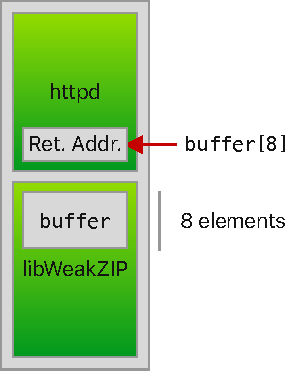
\includegraphics{Images/Buffer Overflow.pdf}
	\end{center}
	\caption{A vulnerability in a (trusted) libWeakZIP procedure may allow an attacker to overflow the stack-allocated buffer. In this example, the return address is stored at the end of the caller's call frame and is thus overwritten by the attack. Note that the stack grows downward.}
	\label{fig:buffoverflow}
\end{figure}

A different but related problem is that adversarial code may ignore the return address provided by the caller and return to a different location within the caller, e.g., skipping an authentication check and jumping straight into the execution path of a successful authentication.

% TODO

\subsection{Proposed Solutions}
A caller can restrict the stack capability before calling a procedure so that the callee only gets access to the unused part of the stack. However, as illustrated in \cref{fig:savedstackcap}, an adversary can save a copy of their stack capability in a first call. If the adversary is called a second time when their stack capability is lower in the stack (due to the stack containing more call frames than during the first call), it can use the saved stack capability to gain access to memory used by other call frames. Several solutions have been proposed to this problem.

\begin{figure}
	\begin{center}
		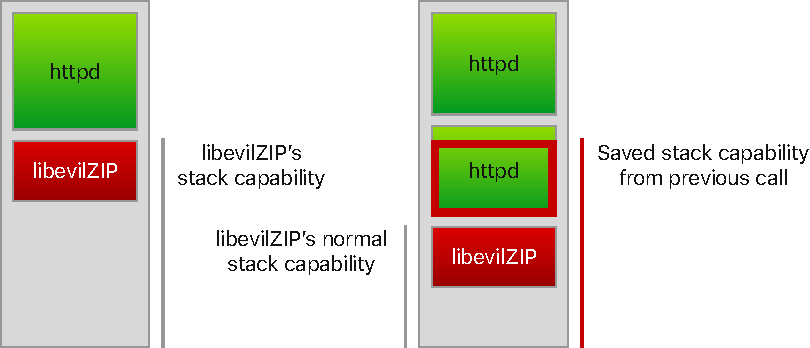
\includegraphics{Images/Saved Stack Cap.pdf}
	\end{center}
	\caption{The call stack in a first invocation (left) and a second invocation (right) of the adversary. During the first invocation, the adversary saves their stack capability for use during a later invocation. Even though the stack capability in the second invocation provides authority over a smaller part of the call stack, the previously saved stack capability continues to provide the adversary with authority over the larger region, which now includes memory occupied by other call frames. Note that the stack grows downward.}
	\label{fig:savedstackcap}
\end{figure}

\paragraph{Using one call stack per compartment} CheriBSD supports compartmentalising software components such that each component gets its own call stack, with the operating system managing a central stack per thread. This approach however requires one call stack per component per thread, one central stack per thread, and one syscall per protection domain transition.\cite{compartment}

\paragraph{Using linear capabilities to restrict copies of the stack capability} The StkTokens calling convention by \cite{stktokens} relies on linear capabilities, a type of capability that can only be moved, not copied. Before calling a procedure, the caller performs a splitting operation which splits the stack capability into two disjoint capabilities. The capability over the caller's call frame is saved whereas the capability over the unused portion of the stack is passed to the callee. The callee returns this capability back to the caller when it returns control to the caller, thereby ensuring that the callee no longer has access to (any portion of) the call stack. The caller merges its saved stack capability with the received stack capability to get the original stack capability back. Linear capabilities are however as of writing not specified for CHERI-RISC-V.

\paragraph{Using local capabilities to revoke copies of the stack capability} A calling convention proposed by \cite{retptr} relies on local capabilities, a type of capability that can be only kept in registers and stored using capabilities that allow storing local capabilities. Local capabilities in CHERI are capabilities without the \emph{Global} permission, whereas capabilities that can be used to store local capabilities have the \emph{Store local capability} permission.

The calling convention relies on making the stack capability a local capability, thereby limiting the locations where it can be stored. Since stack capabilities need to be saved for procedure calls, the stack capability is also given the \emph{Store local capability} permission, to permit storing the stack capability on the call stack. Assuming no other memory regions are given the latter permission, it suffices to clear the unused part of the stack before passing or returning control. This region can however be large and expensive to clear and requires hardware support to do efficiently.

\paragraph{Using local uninitialised capabilities to revoke copies of the stack capability} A calling convention proposed by \cite{uninitcaps} extends on the aforementioned calling convention but without requiring stack clearing. It instead relies on uninitialised capabilities, a type of capability proposed by \cite{uninitcapss} only allowing loads on an initialised part of its bounds. Storing a datum immediately after the initialised region extends the capability's initialised region to include the newly stored datum. A large region of memory can be marked as uninitialised, effectively making them inaccessible unless overwritten. Uninitialised capabilities are however as of writing not specified for CHERI-RISC-V.

\paragraph{Safely heap-allocating call frames} A calling convention proposed by \cite{cerise} sidesteps the stack capability revocation problem altogether by ensuring that call frames always occupy freshly allocated memory to which certainly no dangling capabilities point. GHSCC adapts this calling convention with some minor differences.

\section{Secure Heap Allocation}
% TODO

\section{Secure Calling}
% TODO

\section{Evaluation}
% TODO

\biblio{}
\onlyinsubfile{\glsaddall\printglossaries}
\end{document}
